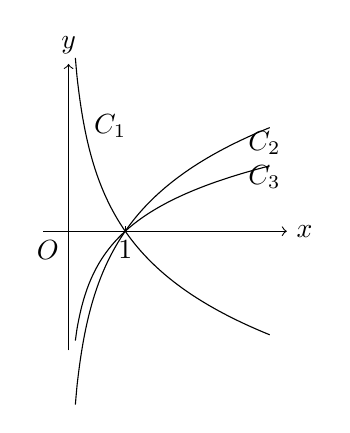
\begin{tikzpicture}[x=.72cm,y=.72cm,baseline=(current bounding box.center)]
  \draw[->] (-.45,0)--(3.85,0) node[right] {$x$}; \draw[->] (0,-2.10)--(0,2.95) node[above] {$y$};
  \draw[domain=.12:3.55,samples=120,smooth] plot (\x,{ln(\x)/ln(.5)});
  \draw[domain=.12:3.55,samples=120,smooth] plot (\x,{ln(\x)/ln(2)});
  \draw[domain=.12:3.55,samples=120,smooth] plot (\x,{ln(\x)/ln(3)});
  \draw (1,0)--(1,.10); \node[below] at (1,0) {$1$}; \node[below left] at (0,0) {$O$};
  \node[right] at (3.00,1.55) {$C_2$}; \node[right] at (3.00,.95) {$C_3$}; \node[right] at (.28,1.85) {$C_1$};
\end{tikzpicture}
